\documentclass{article}
\usepackage{hyperref}
\usepackage{listings}
\usepackage{color}
\usepackage{geometry}
\usepackage{graphicx}
\usepackage{amsmath}
\usepackage{caption}
\usepackage{subcaption}
\geometry{margin=1in}
\pdfminorversion=6

\newcommand\TODO[1]{\textcolor{red}{TODO: #1}}

\newcommand\header[2]{
    \begin{center}
        {\large
        UCSD CSE 272 Assignment #1: \\
        \vspace{0.3cm}
        \Large
        #2}
    \end{center}
}

\definecolor{dkgreen}{rgb}{0,0.6,0}
\definecolor{gray}{rgb}{0.5,0.5,0.5}
\definecolor{mauve}{rgb}{0.58,0,0.82}
\lstset{frame=tb,
        aboveskip=3mm,
        belowskip=3mm,
        showstringspaces=false,
        columns=flexible,
        basicstyle={\small\ttfamily},
        numbers=none,
        numberstyle=\tiny\color{gray},
        keywordstyle=\color{blue},
        commentstyle=\color{dkgreen},
        stringstyle=\color{mauve},
        breaklines=true,
        breakatwhitespace=true,
        tabsize=2
}


\begin{document}

\header{1}{Volumetric Path Tracing}

\begin{figure}[h]
    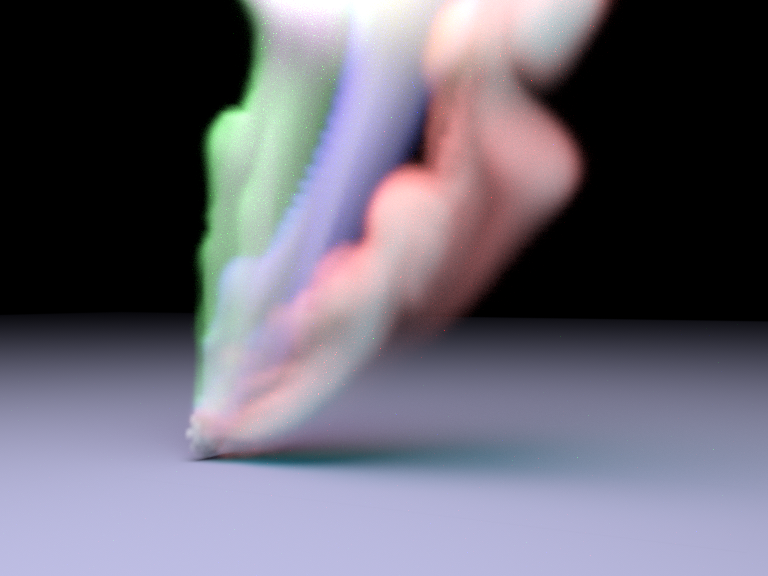
\includegraphics[width=\linewidth]{imgs/colored_smoke.png}
    \caption{A heterogeneous volume with spectrally varying density over space, rendered with multiple-scattering. Smoke data generated using Wenzel Jakob's \href{http://www.mitsuba-renderer.org/misc.html}{fsolver}.}
    \label{fig:gallery}
\end{figure}

In this homework, we will build a volumetric path tracers that can handle scattering and absorption inside participating media inside lajolla. We will split the development into 6 steps and build 6 volumetric path tracers, each has more features than the previous ones.\footnote{This approach is inspired by Steve Marschner's \href{https://www.cs.cornell.edu/courses/cs6630/2015fa/notes/10volpath.pdf}{course note} on volumetric path tracing.} Your $n$-th volumetric path tracer should be able to render all scenes the $(n-1)$-th one can handle.

\end{document}